The system can be calibrated using the GUI for the most common calibration task. Using the config file all parameters are accessable for further calibration.

\subsection{GUI}
A threshold level is used to adjust the system for the current installation height of the camera. It sets a configuration parameter called lowestDistanceOverFloor. This is the limit of how short a person can be. The threshold should be set so that a "normal" person’s chest is not removed by the thresholding.ding.

\begin{figure}[htb]
	\centering
	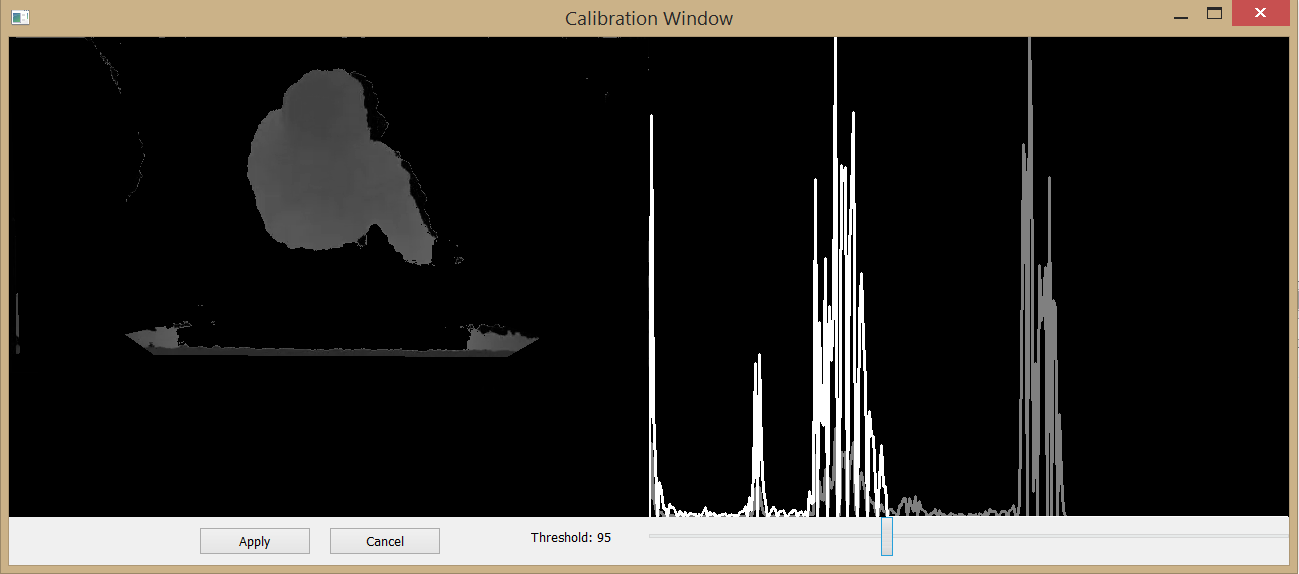
\includegraphics[width=\linewidth]{images/Calibration.png}
	\caption[Overview of the entire system]{\textit{Calibrating the lowestDistanceOverFloor threshold. A histogram i shown to help the user to se how much off different heights are present in the image. The selected heights are gray shaded.}}
	\label{fig:lowestDistanceOverFloor_calibration}  %Skapar referens till figuren
\end{figure}

\newpage
\subsection{Config file}
The config file used by the algorithm pipeline is called \textit{dense\_conf.yml}. In it any configurable variable in any algorithm currently selected to be in the pipeline can be specified. The pipeline itself can also be specified, allowing fo rapid swapping of algorithms. The most useful variables in the current pipeline are shown in table \ref{table:commonVariables}.\\

\begin{table}[hbt]
	\begin{tabular}{ | l | l | p{7.5cm} | }
	    \hline
	    \textbf{Variable} & \textbf{Algorithm/Program-part} & \textbf{Description} \\ \hline
	    runFromFile & Network & If set to 1, the video sources are files found in the paths \textit{videoFilePaths}.  \\ \hline
	    videoFilePaths & Network & The paths to the video files used if running from file.  \\ \hline
	    useKinect & Network & If set to 1, the video sources are from Microsof Kinect cameras. \\ \hline
	    TrackingMaximumDistance & Tracking & The maximum distance a object can be considered to have moved since last frame. \\ \hline
	    TrackingMinimzumLifeSpan & Tracking & The minimal time (in \# frames) a potential object must have existed (and been tracked) before it is considered a real object. \\ \hline
	    TrackingMaximumTimeLost & Tracking & The maximum time (in \# frames) a object is allowed to be lost before it is forgotten. \\ \hline
	    lowestDistanceOverFloor & Kinect Segmentation & The limit (height units) of how short a person can be. Set this variable using the GUI calibration utility described previously. \\ \hline
	    webServerUrl & Network & The address to the web service to which results are reported. \\ \hline
	\end{tabular}
	\label{table:commonVariables}
	\caption{The most useful and common variables in the current pipeline.}
\end{table}

\newpage
Currently the pipeline consists of two major algorithms: \textit{ImageProcessor} and \textit{Analytics}. These in turn have several sub-algorithms that are executed in the order specified in the config file. The current pipe line is structured in the following way: \\
\hspace*{0.5cm}\textit{ImageProcessor:\\
\hspace*{1cm}- KinectSegmentation\\
\hspace*{1cm}- TrackingBruteForce}\\
\hspace*{0.5cm}\textit{Analytics:\\
\hspace*{1cm}- EntryExitCounter\\
\hspace*{1cm}- FlowEstimator\\
\hspace*{1cm}- QueDetector\\
\hspace*{1cm}- QueSeverityEstimator}\\\\
 Any algorithm registed in the system can be used as a subalgorithm for any other algorithm, writing in the config file in the same way as with \textit{KinectSegmentation} being a sub algorithm to \textit{ImageProcessor}. To get an empty algorithm place holder any none-registerd algorithm name (or variable name) may be used, such as:\\
\hspace*{0.5cm}\textit{UnregisterdName:\\
\hspace*{1cm}- KinectSegmentation\\
\hspace*{1cm}- ...}\\
It can now be used as a sub-algorithm to another algorithm (or placeholder algorithm):\\
\hspace*{0.5cm}\textit{ImageProcessors:\\
\hspace*{1cm}- UnregisterdName\\
\hspace*{1cm}- ...}\\
A placeholder algorithm works bu just passing though initialization and processing calls to its sub-algorithms.\\\\
\textbf{Warning: If you do not know what your are doing, don't modify the algorithm pipeline. Some algorithms have requirements which must be provided by earlier algorithms, the system will not run if these aren't met. See the code documentation for further details on requirements and effetcs of different algorithms.}

